% !TeX root = ../main.tex
\section{Study area and data}
\label{sec:materials}

\subsection{Study area and BALSA plantation inventory}
\label{sec:study_area_inventory}

The study covered mainland Ecuador, with particular emphasis on the humid Pacific lowlands and western Andean foothills where commercial BALSA plantations are concentrated as shown in Fig.~\ref{fig:study_area}. Balsa plantation boundaries were obtained from the Ecuadorian Ministry of Agriculture and Livestock through the Geoportal del Agro Ecuatoriano (\url{https://geoportal.agricultura.gob.ec/}).

\begin{figure}[pos=!htbp]
    \centering
    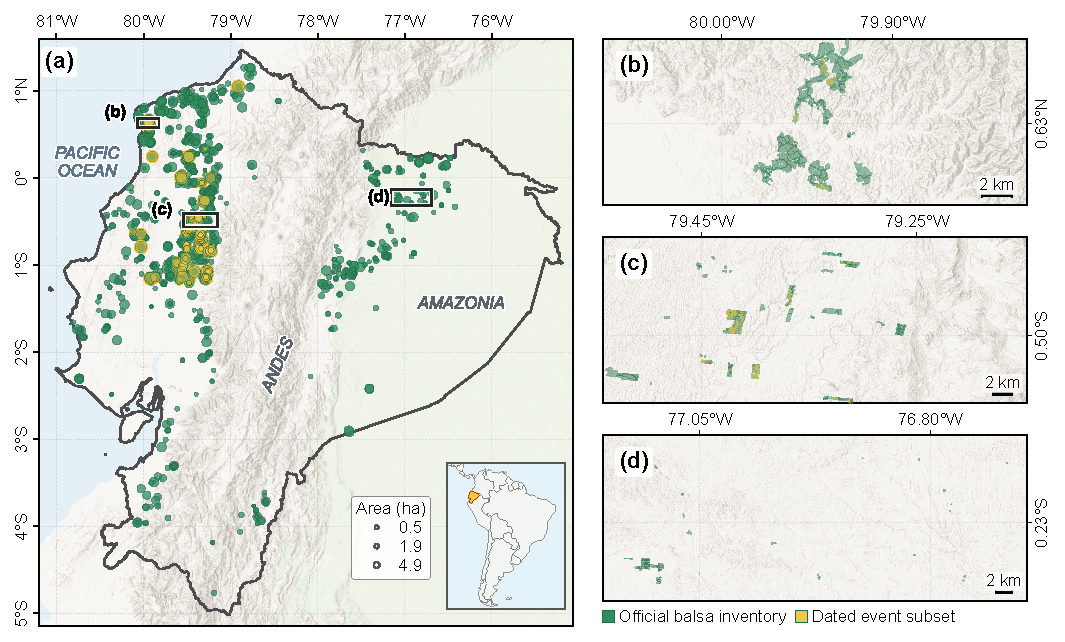
\includegraphics[width=0.92\linewidth]{figures/fig02_study_area.pdf}
    \caption{Study region and official BALSA plantation inventory. Green markers show all 3,890 BALSA polygons, and yellow markers identify the subset containing dated stand-disturbance events. Panels (b)--(d) enlarge representative plantation regions.}
    \label{fig:study_area}
\end{figure}

The source forestry inventory contained 26,206 plantation polygons, of which 3,498 carried the species label BALSA and marked VALIDADO. The validated balsa inventory covered 13,651.85~ha and was divided into three fixed size classes for stratified reporting: small ($\leq1$~ha), medium ($>1$--5~ha), and large ($>5$~ha) (Table~\ref{tab:inventory}).

\begin{table}[pos=!htbp]
    \centering
    \caption{Polygon counts and mapped area by size class for the 3,498 validated BALSA plots in UTM zone 17S (EPSG:32717).}
    \label{tab:inventory}
    \begin{threeparttable}
    \begin{tabular}{lrrrrr}
        \toprule
        Class & Polygons & Polygons (\%) & Area (ha) & Area (\%) & Median (ha) \\
        \midrule
        Small ($\leq1$ ha) & 1,325 & 37.88 & 497.38 & 3.64 & 0.30 \\
        Medium ($>1$--5 ha) & 1,385 & 39.59 & 3,556.10 & 26.05 & 2.33 \\
        Large ($>5$ ha) & 788 & 22.53 & 9,598.37 & 70.31 & 8.68 \\
        \midrule
        Total & 3,498 & 100.00 & 13,651.85 & 100.00 & -- \\
        \bottomrule
    \end{tabular}
    \end{threeparttable}
\end{table}


\subsection{Sentinel-1 OPERA RTC-S1 archive and analytical coverage}
\label{sec:s1_archive}

Sentinel-1 observations were obtained from the NASA OPERA Level-2 Radiometric Terrain Corrected Sentinel-1 (RTC-S1) archive~\citep{shiroma2023OPERARTC,opera2023rtc} and organized using S1-GRiTS v3.0.0 (\url{https://github.com/ottoKae/S1-GRiTS}). OPERA RTC-S1 provides burst-based, radiometrically terrain-corrected $\gamma^{0}$ backscatter at 30-m pixel spacing for VV and VH polarizations.

The Sentinel-1SAR archive in Ecuador contained four relative Sentinel-1 tracks in ascending orbit (TK18, TK47, TK91, and TK120). Native observations began between May and October 2016, depending on the tile--track combination. Observations were indexed on a common monthly calendar from January 2016 to June 2026 while preserving each track's native temporal support; months before a track's first observation or after its final observation remained missing. The historical evaluation interval was fixed to January 2017--December 2025, while observations outside this interval provided temporal context for the windowed detector and the subsequent prospective replay.

The 3,498 validated BALSA polygons intersected 40 tile--track combinations, yielding 4,001 polygon--track objects for time-series extraction. Track identity was preserved throughout time-series construction and disturbance detection so that observations from different relative orbits or viewing geometries were not mixed before event consolidation. Detailed acquisition-level compositing, missing-data handling, and stand-level aggregation are described in Section~\ref{sec:s1_timeseries_representation}.


\subsection{Historical disturbance dated-reference}
\label{sec:historical_references}

Historical disturbance months were assigned by visual interpretation and reconciled to the frozen polygon identifiers. Single-date PlanetScope imagery (approximately 3~m) was the primary evidence source, with monthly Planet basemaps (approximately 4.77~m at the Equator) used where appropriate (Fig~\ref{fig:s1_population_signatures}). Orbit-specific Sentinel-1 observations provided supplementary evidence when cloud cover or incomplete optical observations prevented an unambiguous optical-only date assignment. Interpretation was performed without access to Windowed CUSUM predictions, and ambiguous disturbance dates were not forced into the reference catalogue. After exact polygon--month duplicates were reconciled, the historical catalogue contained 1,093 reference-dated events in 462 validated BALSA polygons distributed across 57 spatial blocks within the 2017--2025 historical evaluation period.

